%In order to sail properly and make the most out of the wind that’s is supplied by the nature itself some data acquisition is needed. The sailing is all about this harnessing all the forces of the nature and the wind that it pushing towards you. Since there has not been any other extensive projects and measurements in this particular area the measurements have to be done in new ways. 
Since all kinds of sailboats main feature is to move completely analogue without the need of fuel or electricity, the use and optimization of surrounding forces are of foremost importance. Measuring this will provide the sailor with all the information needed to optimize the way they move and control their dinghy.

To get any kind of measurements of the dinghy, sensors are needed. As of now there are sensors measuring a wide array of items. This section will talk about these sensors; what they measure, where they were purchased, the requirements on the sensor, their features, drawbacks and also how they were implemented.

\subsection{Force sensors}
The function of the daggerboard is to compensate for the force that the wind is pushing on the sail. The goal is to have a system that can measure the forces that pushes on the daggerboard by the water it goes through. By measuring the side forces on the board, a rough estimation of the exerted force on the sail can be made.  

%The implementation:
\subsubsection{The implementation}
% What is ``this'' approach? Talk first about the approach, then this sentence.
%There might not already be any other solutions as clean and simple as this approach.

% MIN NYA -----------------------------
After some different solutions was suggested the final sensor and measurement method was chosen as the most prominent and clean approach. 
With this implementation the daggerboard itself will not be disassembled or modified in any way. The other solutions are, either way, more difficult to apply and mount or more complex.  
% MIN NYA -----------------------------

%% KANSKE TA BORT
By looking at some different solutions there are no other solutions that might be as clean looking and prominent as this approach. Important to know is that every solution is mandatory to be waterproof and sealed properly from the harsh environment that this system has as its home turf. The solutions that required the sensors to be mounted on the outside or in parts that would be in danger if a crash might occur was scratched.  
The board itself will not be disassembled in any major part of way. Meaning that this approach doesn’t need any modifications to the board itself. This has been the goal and the chosen approach. Modifications in the mounting plate is the way to go, the other solutions is either way more difficult to apply and mount or more complex.
%%% ------------------------------

\subsubsection{The prototype}% If this is about the same as ``Force sensors'', use ``\subsubsection instead.
To implement the gauges, a prototype is designed to show how the measurements will be made. The prototype is a bit bigger than the intended solution for this project but it's good to see how it would be constructed. The function is easy to understand. The board goes on the outside and can easily slide up and down past this ball.  The ball itself is kept inside this small area where it can move in and out.
 
\begin{figure}[H]%look at later figures comment
\begin{center}
	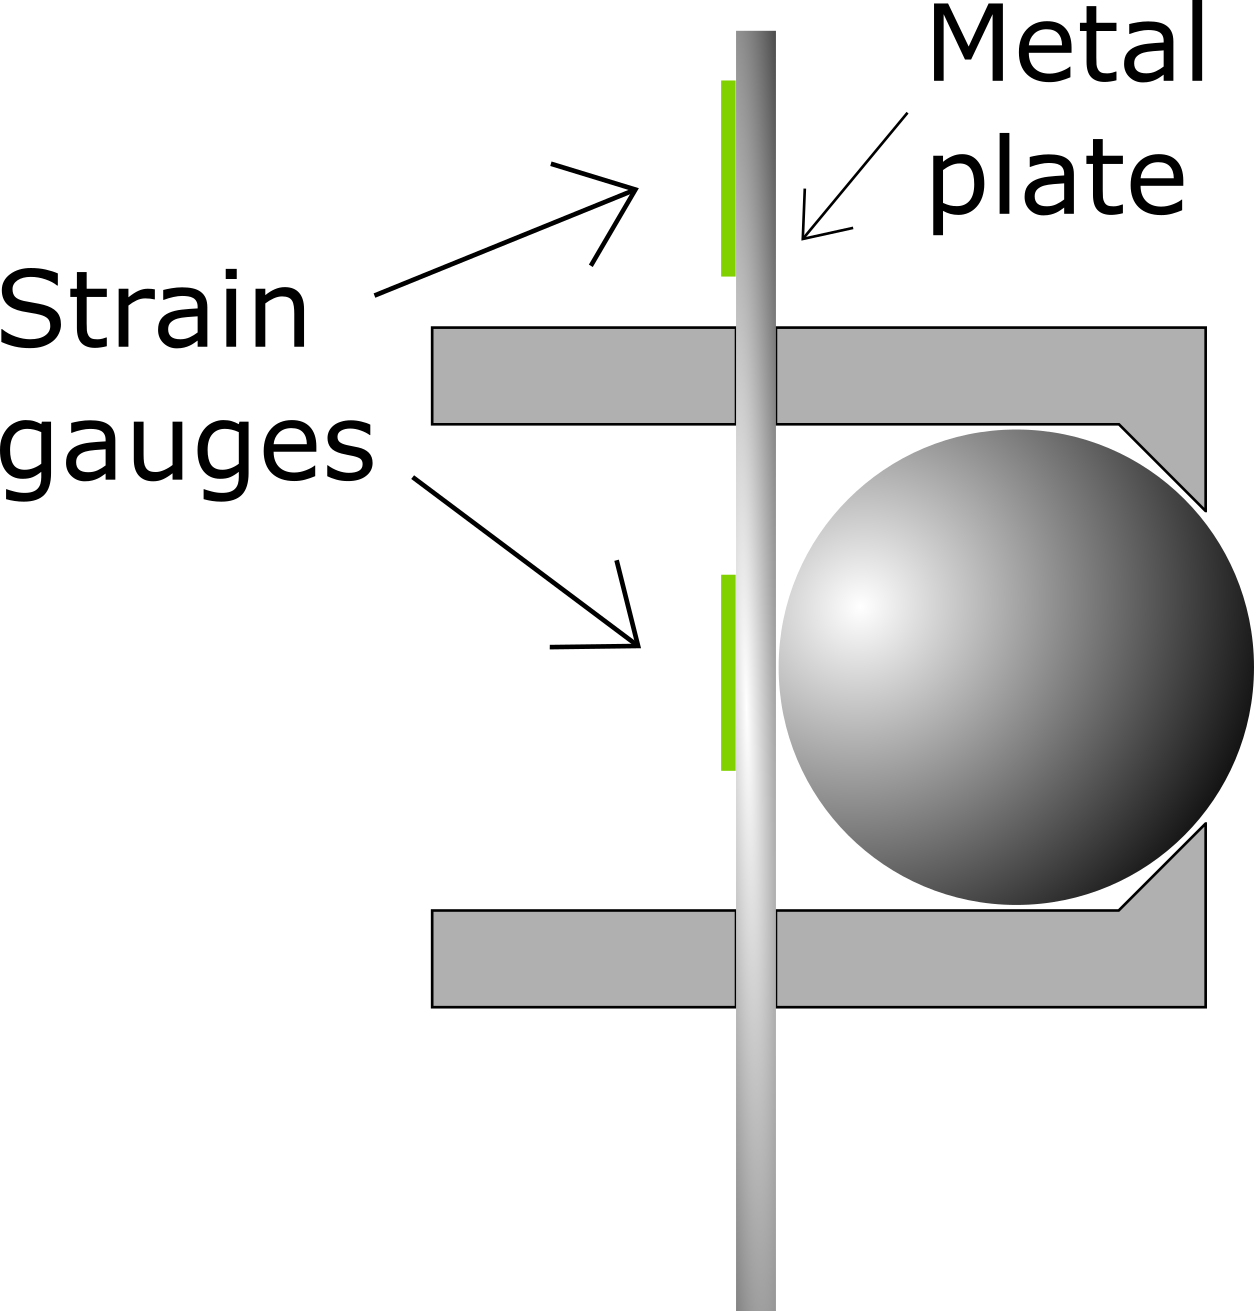
\includegraphics[width = 10cm]{Figures/Press_sens_func_1.png}
	\caption{Function of first prototype}
	\label{Press_sens_prot_1}
\end{center}
\end{figure}

This way of implementing strain gauges was the first idea. 
The main case for this strategy was that in the start of this project these gauges were supplied to us, as a leftover from the last group. With this implementation, we could already start working on a prototype and get a small head start in to the project. But as some research shows, it is a more difficult way to solve this problem and it would take bit more work and some sensitive circuits to measure the force. The gauges also need to be stuck in place using some specific glue and can easily be done incorrectly and therefore prevent good measurements.

A model of the pressure sensor was constructed in the CAD program fusion 3D. This model was created in order to clearly show the function of this sensor and to help the thought process involved in the improving of this design.

\begin{figure}[H]%look at later figures comment
\begin{center}
	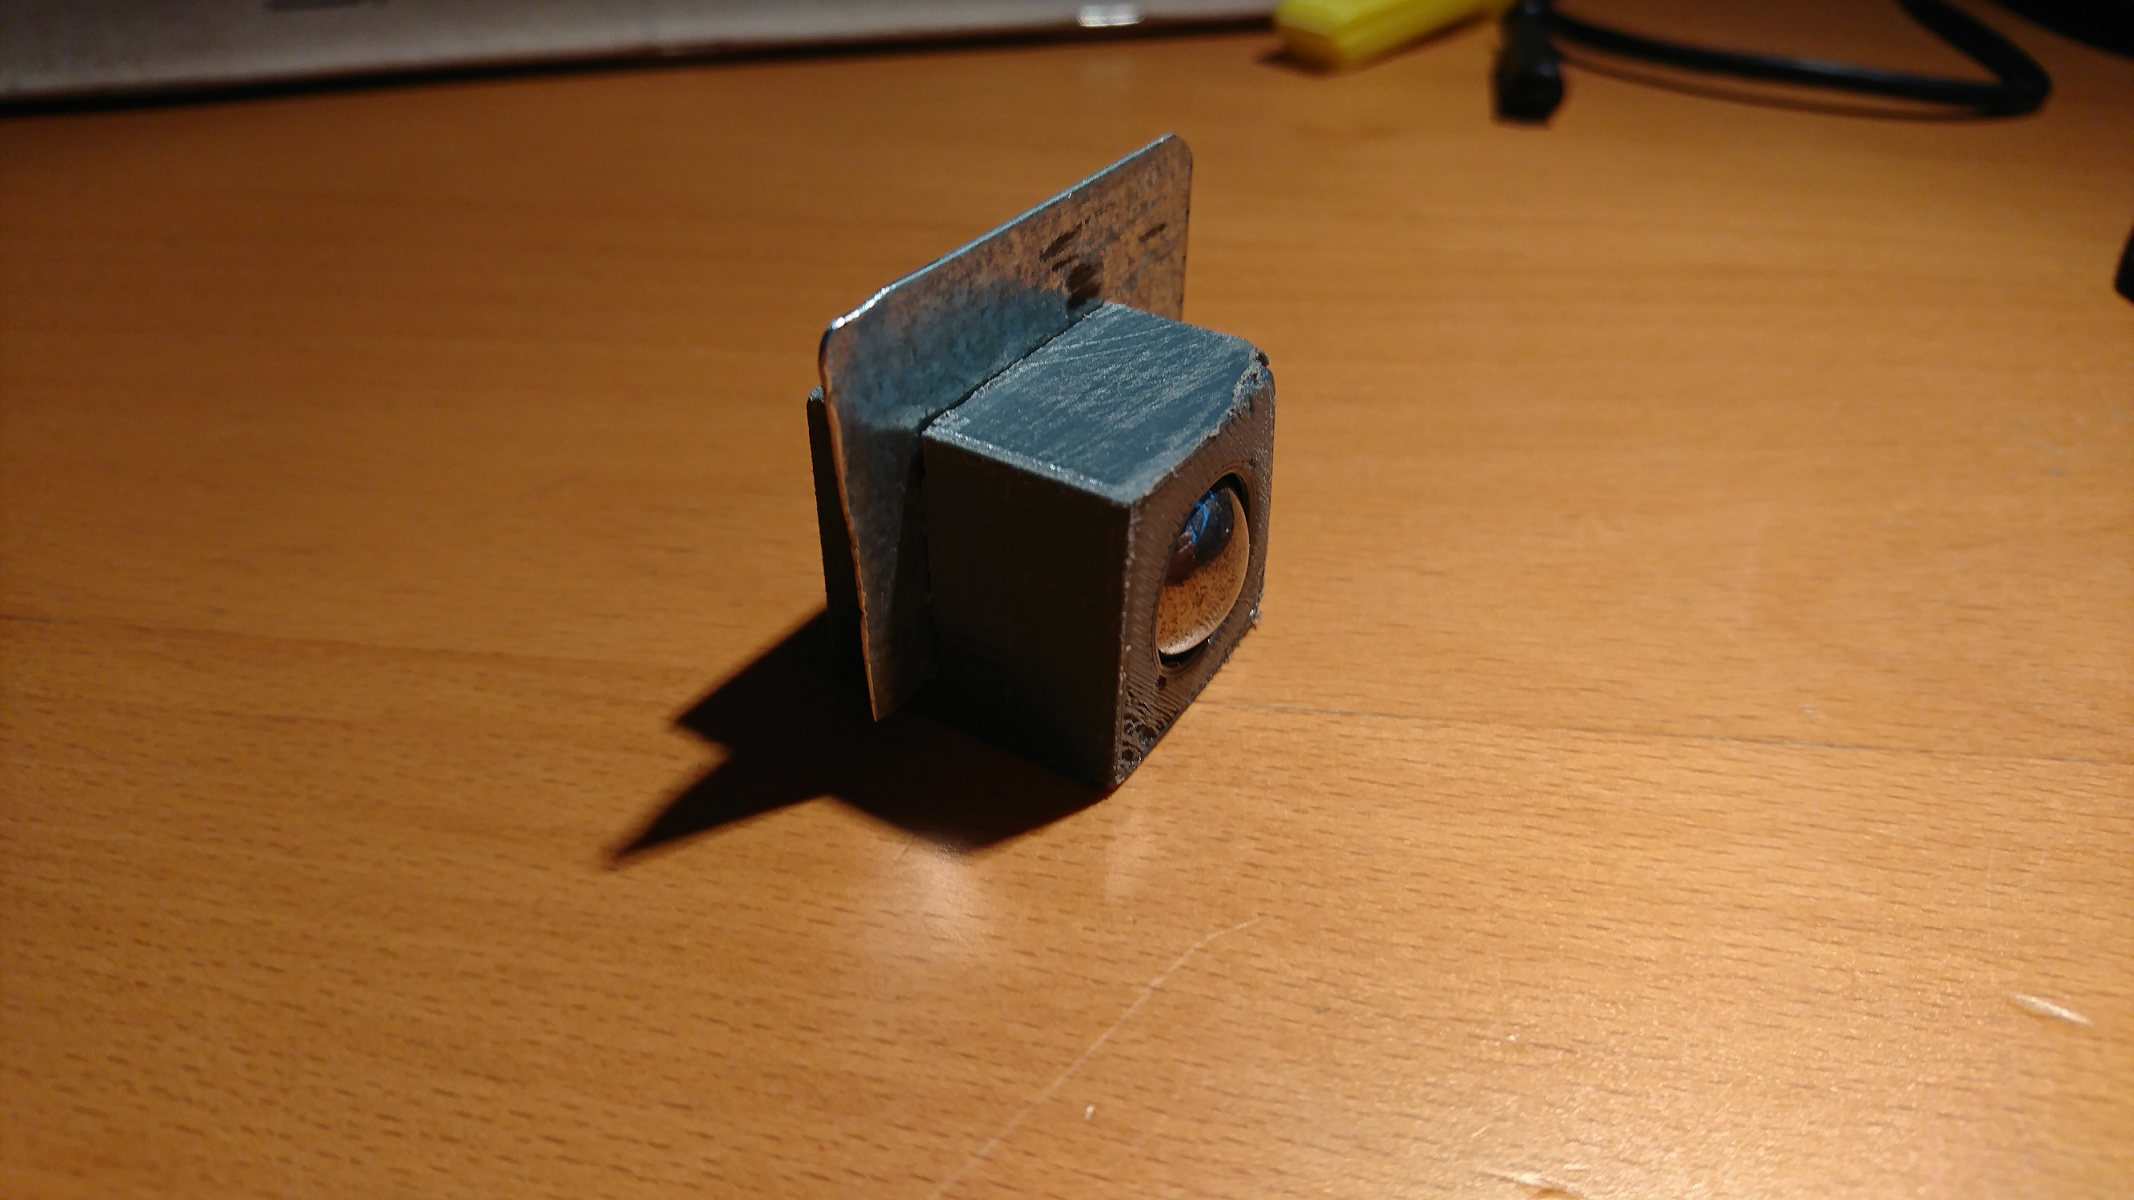
\includegraphics[width = 10cm]{Figures/Press_sens_prot_1.png}
	\caption{Function of first prototype}
	\label{Press_sens_prot_1}
\end{center}
\end{figure}
 The force is then measured at the back where there will be a plate. The deflection of this plate which will be the origin to the strain will be measured through strain gauges. 
The gauge itself will measure a small difference in resistance. This small difference is going to be difficult to measure without any amplifying circuit connected. With a such small signal the system might have issues with noise. Another problem is the signal might drift, and therefore make different measurements as the circuit is running. And finally, with the measured values getting amplified with a big amount the resulting signal may be off by a large amount. 

New idea:
A better solution is to make some research into load cells, which is a sensor which also utilizes strain gauges to measuring forces. The difference is that the gauges are already implemented in the sensor. The difference in the prototype is instead of having a metal plate, it can be built with a piece of plastic or rubber which can deform so the force is distributed directly to the sensor. By implementing this sensor, a lot of time was saved in troubleshooting. And by having a sensor unit, the modified mounting plate will be easier to produce. 
 
\begin{figure}[H]%look at later figures comment
\begin{center}
	
\includegraphics[width = 10cm]{Figures/Press_sens_func_2.png}
	\caption{Function of second prototype}
	\label{Press_sens_prot_2}
\end{center}
\end{figure}

\subsection{Choice of component}

The force from the board onto the mounting plate will be a considerable amount. The actual force is something that’s not known for sure. The initial assumption was that a load cell with a $90.75Kg$ force range should be enough. In the case the sensor will be maxed out the cell it's rated for a $150\%$ overload without causing some damage to the sensor.
The chosen sensor for this application is selected to this part, the compression load cell called FX1901. 
From the datasheet the voltage readings of this piece could be calculated. With a maximum voltage reading of around $36mV/V$

 \begin{figure}[H]%look at later figures comment
\begin{center}
	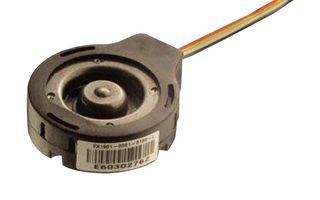
\includegraphics[width = 10cm]{Figures/Load_cell.png}
	\caption{Load cell, FX1901}
	\label{Load_cell}
\end{center}
\end{figure}



\subsection{Amplifier}


In order for the microcontroller to make some good measurements from the load cell an amplification for the  
That’s a small signal and needs to be amplified to get some good measurements. A good measurement signal to the MCU should be in the order of in between $0 - 5$ volts. 
This is achieved by an amplification gain of around $20$. 


A suitable amplifier needs to be chosen from the vast ocean of different models. Inspiration is taken from The university of Chicago\cite{UoC} in an experiment where they uses this exact load cell together with an instrumental amplifier called INA125. This amplifier is somewhat more complicated and have some more features than other amplifiers. %What features? What other amplifiers?
In the same family of instrument amplifiers a model called INA126 is selected as a less complicated and more power efficient solution.


The choice fell on this little fellow, the INA126. %Why is this line here? If this is a reference to a picture make sure to use a reference instead, i.e. "The choice fell on the INA126, see fig. \ref{INA126}, since it best followed our requirements"

\begin{figure}[H]%Make this [tb] and take away [width= X ]  if it is already smaller than \textwidth. Otherwise it will be stretched which will look weird.
\begin{center}
	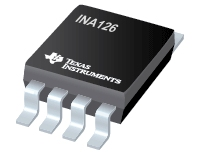
\includegraphics[width = 10cm]{Figures/INA126.png}
	\caption{Amplifier for the load cell signal}
	\label{INA126}
\end{center}
\end{figure}


Which not look so interesting but has the benefit of having a smaller power consumption then many others by being a bit simpler than many others. But sufficient for our purpose.
%Didn't you write in the last paragraph it was power efficient already? And you also wrote it was more complicated and had more features but here you say it's simpler but sufficient? Can this be clarified?

It seems like a smart choice because when the system is battery operated, like in this case, every watt counts.

The gain on this piece is easily calculated with this function. Gain is 5 plus 80k ohm divided by our chosen resistor Rg. % Why write this in plain text when it's already written below? just refer to it!



If our desired 20 gain might not work or the voltages calculated is off, the gain is easily redone with this expression. %It's the same equation...
\begin{equation}%add a \label{labelname} to refer to this equation.
Gain = 5 + \frac{80k\Omega}{R_G}
\end{equation}


Now that we know how to get the force measurements, we are going to talk about how to measure the frequency of waves at sea.


\subsection{Height of centerboard sensor}

The main issues might be that the Height of centerboard: % That the height of the centerboard what?
One of the best implementations of a height sensor would be the use of a linear wire distance sensor. This particular sensor measures how far a wire is pulled, which gives a very accurate measurement. This solution can be completely watertight and concealed in the main centerboard.  

\begin{figure}[H]% As mentioned before, H -> tb, Refer to all figures used, use width only to /restrict/ size.
\begin{center}
	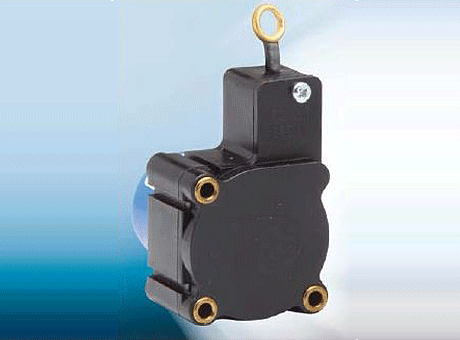
\includegraphics[width = 10cm]{Figures/microepsilon_mk30.png}
	\caption{Linear draw wire sensor, Micro epsilon MK30}
	\label{Draw_sensor}
\end{center}
\end{figure}
 
%Don't use ``this'' without first saying which one. If it's the one in the figure, refer to it by name and then put in a reference to the figure.
%Do not use ``We, us, he, she,...'' and so on in reports. Wold recommend the following:
%The sensor fulfilling our requirements of both functionality and size is the following, NAME, see fig. (\ref{FIGURELABEL}). It is ...
% ``As we have some tight space requirements this can probably fit...'' -> ``As there are some tight space requirements the module needs to fit''
%Avoid all loaded terms and terms that is not objective, such as ``feel like''.
We have found some sensors that might work for us, this is the smallest we found. It is $3cm$ wide and about $5cm$ high. As we have some tight space constraints this can probably fit inside or just stick out a little bit. This particular sensor is in the range of $2000sek$, which feel like a lot. But if no other solution works this might be considered again.  


We have also looked into some light sensors. This is implemented with the use of a plate placed ion top of the dagger-board and with the light being sent up to this panel the height can be calculated. First we looked into some IR\footnote{Infrared}-sensors; they will probably send the signal in a wide spread pattern which will make the distance measurement troublesome as this signal has just a small plate to bounce off of.  
  
%Put all of this paragraph: -->
With the use of a LIDAR\footnote{LIght Detection And Ranging} system, we can point our light signal at an exact spot and then get an exact measurement of the height.  
Many of the LIDAR systems found was both too large and expensive to be implemented in this project.
%Many of the lidar systems we found was too big for our project and also very expensive.  
A suitable small sensor for the Sailoraid system could be the ``micro LIDAR'' circuit from adafruit%\cite{REFERENCE to circuit!}.
%A suitable sensor that we found was a small "micro lidar" circuit from adafruit: 

\subsubsection{Component}% How about: ``$\mu$LIDAR VL53L0X'' ?
% --> here


\begin{figure}[H]
	\centering %\centering can be used inside environments (i.e. all \begin{} here \end{}) and centers everything inside.
	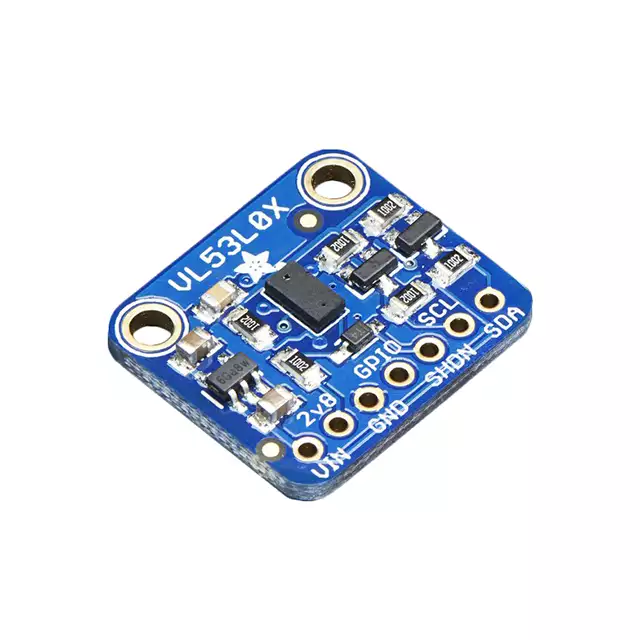
\includegraphics[width = 10cm]{Figures/Adafruit_height_sensor.png}
	\caption{Time of flight, $\mu$LIDAR, distance sensor Adafruit VL53L0X}
	\label{micro_lidar}
\end{figure}
Problems: % Some problems with this module could be compiled. 

As there will always be water around and on the centerplate there is risk of misdirection. The light that is sent might get misdirected if intercepted by water droplets between the sensor and the panel of which the light is to be reflected. %that we want to reflect our light on. 

By the fact that the sensor has to be waterproof the signal has to go through a medium, which can be some type of plastic or even glass.  
If the signal can be read correctly through this medium or if the signal will get corrupted must be further tested. %Remember to print results here later.
%That is something that we need to test later when our parts has come in. 
